\documentclass[12pt, a4paper]{article}
\setlength\parindent{0pt}
\usepackage{polski}
\usepackage[utf8]{inputenc}
\usepackage{fancyhdr}
\usepackage{lastpage}
\usepackage{graphicx}
\usepackage{smartdiagram}
\usepackage{graphicx}

\pagestyle{fancy}
\fancyhf{}
\cfoot{\thepage\ z \pageref{LastPage}}

\lhead{Specyfikacja implementacyjna \textit{Best path} (JAVA)}
\rhead{M.Szlązak, M.Kwiatkowski}


\begin{document}
\title{Specyfikacja implementacyjna programu\\ \textit{Best path} (JAVA)}
\date{15.03.2022}
\author{Michał Szlązak, Maciej Kwiatkowski}
\maketitle
\tableofcontents
\thispagestyle{empty}
\cleardoublepage

\newpage

\setcounter{page}{1}

\section{Cel Projektu}
Celem projektu \textit{Best path} jest stworzenie programu wraz z interfejsem graficznym. Program będzie w stanie wygenerować oraz wyświetlić graf, znaleźć najkrótszą ścieżkę pomiędzy dwoma wybranymi wierzchołkami. Program umożliwi również wczytanie własnego grafu z pliku, wyeksportowanie grafu do pliku i wiele innych. Bardziej szczegółowe wyjaśnienie jakie funkcje będzie spełniał program, co będzie umożliwiał, jak wygląda graf czy przykładowy plik do wczytania -- można znaleźć w~\texttt{Specyfikacji funkcjonalnej (JAVA).tex}.



\section{Wymagania funkcjonalne}
Wymagania funkcjonalne programu przedstawiają jakie funkcje program będzie zawierał po ukończeniu pracy nad projektem.
Program powinien:
\begin{itemize}
\item umożliwić użytkownikowi za pomocą interfejsu:
    \begin{itemize}
        \item wybór czy użytkownik chce wygenerować graf czy wczytać go z~pliku,
        \item podanie nazwy pliku z grafem, który ma być wczytany,
        \item wybór rozmiaru grafu, gdy jest on generowany przez program,
        \item wybór zakresu wag krawędzi, gdy graf jest generowany przez program,
        \item wybór dowolnej ilości par wierzchołków dla których program znajdzie najkrótszą ścieżkę. Dla każdej znalezionej ścieżki możliwa będzie zmiana koloru wyświetlania czy widoczności danej ścieżki,
        \item wybór jednego z trzech trybów działania programu, gdy graf jest generowany przez przez program:
        \begin{itemize}
            \item \texttt{drawing weights}: wszystkie krawędzie między wierzchołkami istnieją, wygenerowane będą losowe wagi z wczytanego zakresu,
        	\item \texttt{drawing weights and edges (graph consistent)}: losujemy czy istnieją krawędzie między wierzchołkami do momentu aż powstanie graf spójny (graf jest spójny gdy dla każdego wierzchołka możemy znaleźć drogę), losujemy wagi z~wczytanego zakresu,
        	\item \texttt{drawing weights and edges (graph not consistent)}: losujemy czy istnieją krawędzie między wierzchołkami, natomiast graf nie musi być spójny, losujemy wagi z wczytanego zakresu,
        \end{itemize}
        \item wybór jednego z dwóch trybów wyświetlania:
        \begin{itemize}
            \item \texttt{basic: }podświetlanie krawędzi oraz wierzchołków przez które przechodzi najkrótsza ścieżka,
            \item \texttt{extended: }podświetlanie krawędzi i wierzchołków przez które przechodzi najkrótsza ścieżka oraz wyświetlanie wag krawędzi przez króre przechodzi ścieżka (wagi będą wyświetlane tylko przy odpowiednim przybliżeniu grafu, w celu zapewnienia czytelności wyświetlanego grafu),
        \end{itemize}
        \item wyświetlenie instrukcji za pomocą przycisku \texttt{help} znajdującym się w pasku menu,
        \item zapisanie wygenerowanego przez program grafu do pliku wybarnego przez użytkownika,
    \end{itemize}
    \item sprawdzić wczytane dane (umożliwić ponowne wprowadzenie danych gdy zajdzie taka potrzeba),
    \item sprawdzić spójność grafu (przy wybraniu trybu trzeciego program powinien wyświetlić komunikat w przypadku gdy użytkownik chce znaleźć ścieżkę pomiędzy wierzchołkami między którymi tej ścieżki nie ma),
    \item znaleźć najkrótszą ścieżkę pomiędzy wybranymi wierzchołkami (o ile taka istnieje) oraz wyświetlić ją na ekranie,
    \item wyświetlić odpowiednie komunikaty w przypadku podania złych danych.
\end{itemize}

\section{Wymagania niefunkcjonalne}
Wymagania niefunkcjonalne to wymagania wobec programu, które nie spełniają funkcji użytkowych dla użytkownika.\\\\
Wymagania niefunkcjonalne wobec programu \texttt{Best Path (JAVA)}: 
\begin{itemize}
    \item program powinien wykryć każdy błąd, który mógłby spowodować niepoprawne działanie programu -- tj. powinien być odporny na błędy ze strony użytkowika,
    \item program powinien być prosty i jednoznaczny w obsłudze -- komenda \texttt{help} powinna w nieskomplikowany sposób wytłumaczyć do czego służy aplikacja, w jaki sposób ją uruchomić, jakie ma możliwości,
    \item program tworzony była na Java 11, dlatego zalecanym jest uruchamianie go na tej właśnie wersji. W przypadku innych wersji może wystąpić problem podczas uruchamiania aplikacji,
\end{itemize}

\section{Diagram modułów}

\begin{center}
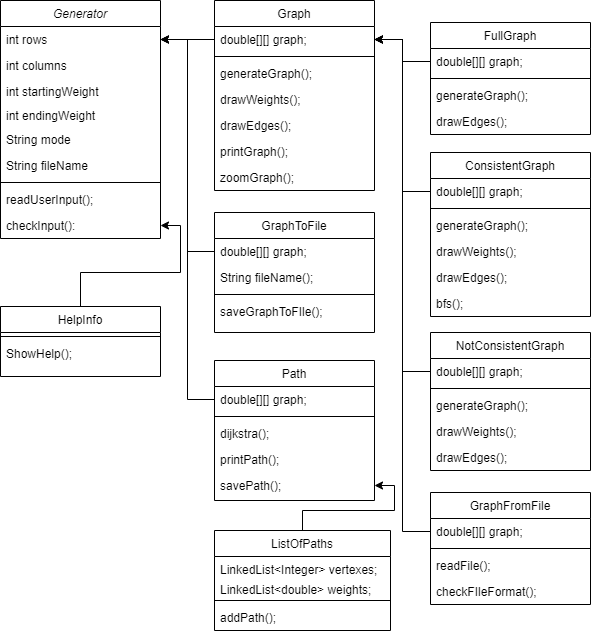
\includegraphics[width=1.1\textwidth]{JIMP JAVA/JIMP Java.png}
\caption{\textit{rys. 1 -- diagram modułów} \label{overflow}}
\end{center}

\textit{Rysunek 1} przedstawia zależności pomiędzy klasami. Przedstawia w jaki sposób został podzielony program, na jakie części, do czego służą dane części programu i w jaki sposób te części są ze sobą powiązane.\\

\textbf{Opis diagramu poszczególnych klas przedstawionych na diagramie (jest to opis ogólny, opis szczegółowy znajduje się w podpunkcie 5 - \textit{Opis modułów i ich funkcji}):}

\begin{itemize}
    \item Klasa \texttt{Generator} to klasa, która będzie odpowiadała za wyświetlenie i~obsługę interfejsu graficznego. Jest również odpowiedzialna za uruchamianie opowiednich metod w zależności od tego co w danym momencie będzie robił użytkownik.
    \item Klasa \texttt{Graph} to klasa, która będzie odpowiadała za stworzenie grafu oraz wyświetlenie grafu. Jest to klasa abstrakcyjna, metoda \textit{generateGraph} jest zależna od tego jaki tryb generowania grafu wybierze użytkownik (lub gdy użytkownik wybierze wczytywanie grafu z pliku).
    \item Klasy \texttt{FullGraph, ConsistentGraph, NotConsistentGraph, GraphFromFile} to klasy, które definiują działanie metody \textit{generateGraph} w zależności od tego jaki tryb generowania grafu wybierze użytkownik.
    
    \begin{itemize}
        \item \texttt{FullGraph} jest uruchamiany gdy losujemy jedynie wagi w wybranym przedziale.
        \item \texttt{ConsistentGraph} jest uruchamiany gdy losujemy wagi (w wybranym przedziale) oraz krawędzie -- a wygenerowany graf ma być spójny (z każdego dowolnego wierzchołka istnieje droga do każdego innego wierzchołka). Spójność jest sprawdzana za pomocą  metody \texttt{bfs}, która wykorzystuje algorytm bfs.
        \item \texttt{NotConsistentGraph} jest uruchamiany gdy losujemy wagi (w wybranym przedziale) oraz krawędzie -- a wygenerowany graf nie musi być spójny.
        \item \texttt{GraphFromFile} jest uruchamiany gdy użytkownik chce wczytać graf za pomocą pliku.
    \end{itemize}
    \item \texttt{GraphToFile} to klasa, która służy do zapisywania grafu do pliku.
    \item \texttt{Path} to klasa, która odpowiada za znalezienie oraz wyświetlenie najkrótszej ścieżki pomiędzy wierzchołkami wybranymi przez użytkownika. Ścieżka zostanie znaleziona za pomocą algorytmu Dijkstry.
    \item \texttt{ListOfPaths} to klasa, która odpowiada za zapisywanie znalezionych ścieżek w celu swobodnego ich wyświetlania i chowania w zależności od wyborów użytkownik.
    \item \texttt{HelpInfo} to klasa, która odpowiada za wyświetlanie informacji dotyczących działania programu, gdy użytkownik wybierze taką opcję.
\end{itemize}



\section{Opis klas i ich metod}
Klasy w programie odpowiadają za działanie programu, znajduje się w nich kod wszystkich metod potrzebnych do działania programu.

\subsection{Generator.java}
W klasie \texttt{Generator.java} będzie główna część programu -- w nim wywoływane będą metody z pozostałych klas. Będzie odpowiedzialny za monitorowanie działania użytkownika i wykonywanie odpowiednich metod w zależności od tego jakie działania zostały podjęte. Odpowiada również za wyświetlenie i ustawienia GUI. Będzie wczytywać i sprawdzać dane wprowadzone przez użytkownika do programu.\\\\
Metody znajdujące się w klasie \texttt{Generator.java}:
\begin{itemize}
    \item Główna metoda \texttt{main.java}: \texttt{public static void main(String[] args)}\\
    Zmienna \texttt{args} pozwala przechowywać dane podane przy uruchamianiu    programu, natomiast nie będzie ona używana,
    \item \texttt{public void checkInput()} -- metoda sprawdzająca poprawność podanych danych,
    \item \texttt{public void readUserInput()} -- metoda wczytująca dane podane przez użytkownika.
\end{itemize}

\subsection{Graph.java}\\\\
Klasa \texttt{Graph.java} będzie klasą abstrakcyjną, zawierającą metody pozwalające stworzyć graf według danych podanych przez użytkownika poprzez GUI. Do tego będą potrzebna metody:
\begin{itemize}
    \item \texttt{public double[][] generateGraph(int mode, int start\_weight, int end\_weight, int rows, int columns)} -- która pozwoli mu zaalokować pamięć dla grafu. Zmienne \texttt{columns} i \texttt{rows} przyjmują wartości $<2,1000>$.
    \item \texttt{public void drawWeights (double[][] graph, int startWeight, int endWeight, int rows, int columns)} -- która będzie losowała wagi dla każdej krawędzi.
    \item \texttt{public void draw\_edges (double[][] graph, int rows, int columns, int chance)} -- która będzie losowała istnienie krawędzi (nieistniejące krawędzie będą miały wartość -1).
    \item \texttt{public boolean BFS (double[][] graph, int rows, int columns)} -- która pozwoli stwierdzić spójność grafu. Zwraca: wartości \texttt{0} -- gdy graf jest spójny, \texttt{1} -- gdy graf jest niespójny.
    \item \texttt{public void printGraph(double[][] graph)} -- która narysuje graf w przeznaczonym na to panelu.
\end{itemize}

Wyjaśnienie znaczenia zmiennych występujących w metodach: 
\begin{itemize}
    \item \textit{graph} -- tablica dwuwymiarowa zawierająca informacje na temat wag krawędzi wychodzących z danego wierzchołka. Jest to tablica o wymiarach [n][4], gdzie n to liczba wierzchołków. Wartość [n][0] przechowuje informacje na temat wagi krawędzi prowadzącej w górę. Wartość [n][1] przechowuje informacje na temat wagi krawędzi prowadzącej w dół. Wartość [n][2] przechowuje informacje na temat wagi krawędzi prowadzącej w prawo. Wartość [n][3] przechowuje informacje na temat wagi krawędzi prowadzącej w lewo. Jeżeli tablica przechowuje wartość -1 to znaczy że dana krawędź nie istnieje.
    \item \textit{rows, columns} -- zmienne całkowite odpowiadające liczbie rzędów i kolumn w grafie.
    \item \textit{int mode} -- tryb uruchomienia programu.
    \item \textit{int start\_weight} -- początek przedziału wag ścieżek.
    \item \textit{int end\_weight} -- koniec przedziału wag ścieżek.
    \item \textit{chance} -- szansa na usunięcie krawędzi (przydaje się gdy generujemy graf spójny i chcemy za każdym nieudanym generowaniem zwiększyć szansę osiągnięcia sukcesu).
\end{itemize}

\subsection{FullGraph.java}
Będzie to klasa roszerzona o klasę abstrakcyjną \texttt{Graph}, za pomocą której stworzony będzie graf, w którym każdy wierzchołkem ma połączenie do sąsiadującego wierzchołka. Do tego potrzebne będą metody:
\begin{itemize}
    \item \texttt{public double[][] generateGraph(int mode, int start\_weight, int end\_weight, int rows, int columns)}.
    \item \texttt{public void draw\_edges (double[][] graph, int rows, int columns, int chance)}.
\end{itemize}
Opisy podanych metod znajdują się w sekcji 5.3.

\subsection{ConsistentGraph.java}
Będzie to klasa roszerzona o klasę abstrakcyjną \texttt{Graph}. Będzie ona odpowiadać za stworzenie spójnego grafu. Wykorzystane zostaną do tego metody:

\begin{itemize}
    \item \texttt{boolean bfs (double[][] graph)} -- zwraca wartości \texttt{true} -- gdy graf jest spójny, \texttt{false} -- gdy graf nie jest spójny.
    \item \texttt{public double[][] generateGraph(int mode, int start\_weight, int end\_weight, int rows, int columns)}.
    \item \texttt{public void draw\_edges (double[][] graph, int rows, int columns, int chance)}.
    \item \texttt{public void drawWeights (double[][] graph, int startWeight, int endWeight, int rows, int columns)}.
\end{itemize}

Opis metody \texttt{bfs}:\\
Dla każdego wierzchołka grafu (dla każdego po kolei od 0 -- n) będzie szukał połączenia z najbliższymi wierzchołkami (najbliższy wierzchołek -- taki od którego dzieli tylko jedna krawędź) i dodawał je do kolejki ,,queue". Wierzchołek dla którego znaleziono już wszystkie najbliższe połączenia trafia na listę ,,visited" (tj. odwiedzone -- takie do których da się dotrzeć). Następnie zostaje usunięty z kolejki ,,queue". Dla każdego następnego wierzchołka w kolejce wyszukuje wszystkie najbliższe połączenia z innymi wierzchołkami, dodaje te wierzchołki do kolejki (o ile jeszcze ich tam nie ma). Gdy już wszystkie najbliższe połączenia dla następnego wierzchołka zostały znalezione i dodane do kolejki, dodaje ten wierzchołek do listy ,,visited", usuwa z~kolejki ,,queue", powtarza te czynności aż kolejka ,,queue" będzie pusta. Jeżeli na liście ,,visited" znalazły się wszystkie wierzchołki -- to oznacza, że graf jest spójny -- dla sprawdzonego w danym momencie wierzchołka. Czynność jest powtarzana aż sprawdimy wszystkie wierzchołki.\\
Metodę można usprawnić, kończąc sprawdzanie spójności dla danego wierzchołka gdy dotrzemy z niego do innego wierzchołka, który już został sprawdzony (jeżeli wierzchołek o indeksie \textit{1} został już sprawdzony i jest spójny, a~więc można z niego dotrzeź do każdego innego wierzchołka, to ze sprawdzanego wierzchołka \textit{4} dotrzemy do wierzchołka \textit{1} -- to kończymy dalsze sprawdzanie, poniewaź z wierzchołka \textit{1} można dotrzeć do każdego innego wierzchołka).\\\\
Opisy pozostałych metod znajdują się w sekcji 5.3.

\subsection{NotConsistentGraph.java}
Klasa ta będzie roszerzona o klasę abstrakcyjną \texttt{Graph}. Klasa ta będzie miała za zadanie wygenerowanie grafu, który nie musi być spójny.
W tym celu potrzebne będą metody:

\begin{itemize}
    \item \texttt{public double[][] generateGraph(int mode, int startWeight, int endWeight, int rows, int columns)}.
    \item \texttt{public void draw\_edges (double[][] graph, int rows, int columns, int chance)}.
    \item \texttt{public void drawWeights (double[][] graph, int startWeight, int endWeight, int rows, int columns)}.
\end{itemize}
Opisy podanych metod znajdują się w sekcji 5.3.

\subsection{GraphFromFile.java}
Klasa ta będzie zawierała metodę czytającą plik z grafem podanym przez użytkownika oraz będzie zawierała metodę sprawdzającą format danych podanego pliku. \\
\begin{itemize}
    \item \texttt{public boolean checkFileFormat (string filename)} -- funkcja sprawdzająca format danych. Zwraca: \texttt{true} -- gdy format jest poprawny, \texttt{false} -- gdy format jest niepoprawny.
    \item \texttt{double[][] readFile (string filename)} -- Funkcja czytająca dane z pliku. Zwraca stworzony graf.
\end{itemize}

Wyjaśnienie znaczenia zmiennych występujących w metodach:
\begin{itemize}
    \item \textttt{string filename} -- nazwa pliku do otwarcia 
\end{itemize}

\subsection{GraphToFile.java}
Klasa ta będzie zawierała metodę czytającą plik z grafem podanym przez użytkownika oraz będzie zawierała metodę sprawdzającą format danych podanego pliku. \\
\begin{itemize}
    \item \texttt{public boolean checkFileFormat (string filename)} -- funkcja sprawdzająca format danych. Zwraca: \texttt{true} -- gdy format jest poprawny, \texttt{false} -- gdy format jest niepoprawny.
    \item \texttt{double[][] readFile (string filename)} -- Funkcja czytająca dane z pliku. Zwraca stworzony graf.
\end{itemize}

Wyjaśnienie znaczenia zmiennych występujących w metodach:
\begin{itemize}
    \item \textttt{string filename} -- nazwa pliku do otwarcia.
\end{itemize}

\subsection{Path}
Klasa \texttt{Path} odpowiada za znalezienie najkrótszej ścieżki pomiędzy wierzchołkami wybranymi przez użytkownika. Zostanie to wyonane za pomocą metody \texttt{dijkstra}. Znaleziona ścieżka zostanie wyświetlona za pomocą metody \texttt{printPath}, która będzie brała pod uwagę kolor, tryb oraz widoczność (czy jest lub nie jest widoczna) wybrane przez użytkownika. Zapisze również znalezioną ścieżkę do klasy listOfPaths.

Metody znajdujące się w klasie:
\begin{itemize}
    \item \texttt{public void dijkstra (double graph[][], int startingVertex, int endingVertex, int rows, int columns)} -- metoda, która znajduje najkrótszą ścieżkę pomiędzy dwoma wierzchołkami.
    \item \texttt{public void printPath(String mode)} -- metoda, która wyświetli znalezioną ścieżkę na grafie.
    \item \texttt{public void savePath()} -- metoda, która zapisze znalezioną ścieżkę oraz wagi krawędzi tej ścieżki.
\end{itemize}


\subsection{ListOfPaths}
Klasa \texttt{listOfPaths} odpowiada za zapisanie ścieżki znalezionej w klasie \texttt{Path} w celu łatwego rysowania i ukrywania ścieżek w GUI. Klasa zawiera jedną metodę \texttt{public void addPath(int[] vertexPath, double[] weightPath);}. Znajdują się w niej dwie tablice \textit{vertexPath oraz weightPath} -- pierwsza zawiera ścieżkę składającą się z indeksów wierzchołków a druga zawiera wagi krawędzi ścieżki. Klasa zawiera dwie zmienne LinkedList które będą przechowywały ścieżki wraz z ich informacjami.



\subsection{HelpInfo.java}
Bedzie to klasa zawierająca metodę odpowiedzialną za wyświetlenie instrukcji obsługi programu:

\begin{itemize}
    \item \texttt{public void showHelp()} -- metoda wyświetlająca instrukcję obsługi programu.
\end{itemize}


\section{Przeprowadzanie testów}
Testy będą automatyczne, przeprowadzane za pomocą Maven'a . Przygotowane zostaną gotowe pliki, które będą uruchamiały program z przygotowanymi danymi i będą porównywać otrzymany wynik z przewidywanym wynikiem. 



\section{Wybrane środowisko}
Środowisko jakie zostanie wykorzystane w trakcie pracy nad projektem to GIT. Biorąc pod uwagę, że pracujemy w grupie potrzebujemy środowiska, które umożliwi nam łatwe i bezpieczne rozgałęzienie pracy -- dlatego wybraliśmy GIT'a.\\\\

Używane środowiska:\\
OS: Windows 11\\
JDK version: JDK 11.0.15\\
Editor: Intellij IDEA Community Edition 2021.3.2, Scene Builder Version 17.0.0\\\\
Parametry komputera:\\
CPU: Intel(R) Core(TM) i7-8750H CPU @ 2.20GHz   2.20 GHz\\
RAM: 2 x 8 DDR4, 8 GB, 2666 MHz

\section{Konwencja wprowadzania zmian}
Pomimo, że projekt nad którym pracujemy nie jest bardzo skomplikowany i~nie powinien być znacząco rozbudowany, każda osoba pracująca nad projektem będzie pracowała na własnej gałęzi, dopiero po sprawdzeniu działania wprowadzonych zmian, zmiany zostaną wprowadzone do gałęzi głównej. W~przypadku takiego projektu tworzenie dodatkowych gałęzi jest niepotrzebne i na tym poziomie wystarczy ograniczenie się do~gałęzi \texttt{Master}. Każda zmiana będzie przejrzyście zakomentowana. W przypadku wprowadzania dużej ilości zmian będą stosowane tagi wg. konwencji (z małymi komentarzami) v1, v2..., wersja końcowa \textit{vn\_FINAL} - gdznie n - to nr. taga.
 
\end{document}


